%\RequirePackage[l2tabu, orthodox]{nag}  %Checks for older packages

\documentclass[11pt,a4paper]{article}
% \documentclass[10pt]{extreport} $ allos to make the font smaller
\usepackage[utf8]{inputenc}

\usepackage{amsmath}
\usepackage{amsfonts}
\usepackage{indentfirst}
\usepackage{amssymb}
\usepackage[font={footnotesize}]{caption} %Makes the captions small

%\usepackage{algorithm}
%\usepackage{algpseudocode}
\usepackage[linesnumbered,ruled,vlined]{algorithm2e}

%% Figures packages
\usepackage[pdftex]{graphicx}
\usepackage{float}   %Es para colocar el objeto flotante exactamente donde se ponga el comando con H
\usepackage{caption}
\usepackage{subcaption}
\graphicspath{{../results/}}
\usepackage{sidecap}  %Para poner figuras a los lados


\usepackage{setspace} % Needed for Pyton syntax highlight
\usepackage{listings}    % Include the listings-package, nice verbatim for code
\usepackage{color}
\usepackage{courier}


\usepackage{cleveref} %puts figure and equation appropiately \cref{}

\usepackage{natbib} %For bibliography
%\usepackage{cite}
\usepackage{framed} % To use boxes, or frames around text

\usepackage{parskip} %Para saltos entre parrafos
\setlength{\parindent}{0pt}
\setlength{\parskip}{\baselineskip}
\usepackage[a4paper,margin=0.8in]{geometry}  %%Cambiar los margenes

\newcommand{\HRule}{\rule{\linewidth}{0.5mm}}
\newcommand{\Wb}{\mathbf{w}}

%\usepackage{hyperref} %This should be loade after most of the other packages
% \hypersetup{colorlinks=true}  %Para que los hiperlinks cuando se hagan referencias aparezcan en colores.



\definecolor{dkgreen}{rgb}{0,0.6,0}

\title{Lab12: DD2380 }
\author{
Ramon Heberto Martinez Mayorquin  hramon@kth.se
Akash Kumar Dhaka  akashd@kth.se
}



\begin{document}

\begin{titlepage}
\begin{center}
%\includegraphics[width=0.15\textwidth]{logo}\\[1cm]

\textsc{\LARGE Kungliga Tekniska högskolan}\\[1.0cm]

\textsc{\Large Summer School: Introduction to High Performance Computing}\\[2.0cm]



\begin{figure}[H]
	\centering
 
\includegraphics[width=0.35\textwidth]{Kth_logo.png}
\end{figure}
%\\[1cm]
%

% Title
\HRule \\[0.4cm]
{ \huge  Project: Stochastic Gradient Descent in CUDA.
}\\[0.4cm]
\HRule \\[1.5cm]

% Author and supervisor

Authors: Ram\'on  Mart\'inez, Theodoros Vasiloudis   \\
\large Professors: One Dude, The other dude.  \\ [2.5cm]
%\normalsize Presenta \\
%\large Supervisors 2: Jan Antolik \\[2.5cm]

\textsc{\Large School of Computer Science and Communication \\
PDC Center for High Performance Computing}\\ [1.0cm]
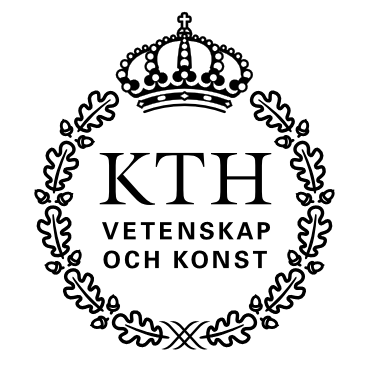
\includegraphics[width=0.15\textwidth]{KTH_black.png}\\[1.5cm] % Controls the distance till the new object
% Bottom of the page
{\large 15 September of 2015}

\end{center}
\end{titlepage}

\begin{abstract}
Parallelize this parallelize that.

\end{abstract}

\section{Stochastic Gradient Descent}

%TODO: (Throughout text) Ensure vectors are typed with \mathbf{v}, have \Wb command for w

One of the most common problems in estimation, optimization theory and machine learning is
minimizing an objective function \citep{bottou2010large}. Consider the \textit{loss} function $Q(z,
w)$. This function depends both on a sample $z=(x, y)$ which is a pair made of an input $x$ and an
output $y$ and on the vector $\Wb$ which parametrizes the function that connects the input to the
output. In such a context we would like to find the vector $\Wb$ that minimizes this error averaged
over our data. In a more mathematical parlance we write that following:

\begin{equation}
E(w) = \frac{1}{n} \sum_{i=1}^n Q(z_i, w)
\end{equation}

where $i$ the sample index, as we go through the complete dataset $\mathbf{z}$.

The Gradient Descent method proposes moving in the direction of the gradient in order to
find $w$. That is, we perform steps of a given size in the direction of the gradient of the loss function and update $w$ at every step:

\begin{equation}
w_{t + 1} = w_t - \gamma \sum_{i=1}^n \triangledown_w Q(z_i, w)
\end{equation}

where $\gamma$ controls the step size. This quantity is usually called the learning rate and
controls the speed or rate of change in $w$. $gamma$ is of crucial importance for the
convergence or divergence of the algorithm, setting $gamma$ too high leads to large changes at each iteration and
making it possible for the algorithm to diverge. If we set $gamma$ too small the algorithm
will not perform enough exploration, leading to slow convergence.

Under sufficient regularity assumptions when the initial estimate of $w$ is close enough to the
minimum and the learning rate is small enough this algorithm can achieve linear convergence
\citep{dennis1996numerical}.

Stochastic Gradient Descent (SGD) is a variation of the scheme proposed above that can be used
when the complete dataset is not available at runtime, e.g. in a streaming setting,
or when the data does not fit into memory.
In this case instead of taking the average gradient over the complete data we only use the local
gradient taken from a single datapoint to calculate the direction of movement:

\begin{equation}
w_{t + 1} = w_t - \gamma  \triangledown_w Q(z_i, w)
\end{equation}

It follows from the algorithm that this optimization can be implemented online due to the fact that
very little memory is needed for the calculation. The convergence of stochastic gradient descent is granted
in  some mild conditions when the learning rate $\gamma$ decreases over time in such a way that the
series  indexed by them does not diverge \citep{bottou2010large}.

In \citep{wilson2003general} it is shown, perhaps counter-intuitively, that batch gradient descent has
worse run-times and convergence characteristics when compared to stochastic gradient descent.

Mini-batch stochastic gradient descent lies somewhere in the middle between these two algorithms.
There, the optimization process is performed on small subsets of the complete dataset that are
called \textit{batches}. At each step in the algorithm we choose a random subset of the data,
calculate the gradient, and update the weights, based on the information we are able to get from
the batch. The main advantage in speed for mini-batch SGD comes from the fact that instead of the
matrix-vector multiplications that are necessary in plain SGD, we are able to batch samples
together and perform matrix-matrix multiplications, thereby allowing for a more efficient learning
process.

\section{Parallel Stochastic Gradient Descent}
\subsection{Related Work}

There exist a number of approaches for parallelizing SGD \citep{zinkevich2010parallelized,
recht2011hogwild, dekel2012optimal}, and each comes with some advantages and disadvantages. Some of
these algorithms are mostly intended to be used in a distributed setting, but can however be
adapted to function well in a highly parallel setting as well.

The approach presented in \citep{zinkevich2010parallelized} is an intuitive parallel extension of
SGD, where each processor solves a local SGD problem using a random partition of the
complete dataset, and the solutions from each processor are then communicated and averaged. This
approach involves practically no communication between the processors during the optimization
phase. While this is beneficial in terms of network/communication costs, it results in subpar
performance when it comes to the optimality of the solution.

\cite{recht2011hogwild} also propose an asynchronous algorithm which is aimed at problems with
sparse parameters, i.e. we assume that the cost function we are optimizing can be decomposed (to a
degree). This property makes it possible for individual processors to work on different parts of
$\Wb$, and perform gradient descent using only a single parameter from the complete weight vector,
making it possible to atomically update that single parameter, in parallel with the other
processors, without the need for locking the weight vector while one processor makes its updates.
While this approach allows for fast iterations since each processor can work and update his part of
the solution independently from the others, it has the additional assumption of problem sparsity
and the lack of communication between processors can often lead to diverging solutions
\citep{dai2015analysis}.

\cite{dekel2012optimal} show a distributed mini-batch SGD approach which they show is optimal in
terms of the \textit{optimality gap} which they define as the difference between the loss given by
the optimal weight vector $Q(z, w^*)$ and the approximation obtained by the algorithm, $Q(z,
\bar{w})$. The algorithm proposed uses mini-batches to calculate approximate gradients for each
processor, which are then summed and averaged across the different processors, and the averaged
gradient is used to update the weights at the end of each iteration. While this algorithm obviously
has higher communication costs when compared to the ones we described before, it can attain better
convergence guarantees, and enjoys faster convergence in terms of number of iterations, as the
different processors have access to more up-to-date and consistent sets of weights. One drawback of
this approach when it comes to highly parallel architectures however is that its parallelization
factor is limited by the minimum of number of batches and available processors.

\subsection{Algorithm Used}

For this work we chose a variant of the algorithm described by \cite{dekel2012optimal}, which involves the following steps:

\begin{enumerate}
	\item  	For each iteration:
	\begin{enumerate}
		\item Shuffle the dataset, and split into batches of size $b$.
		\item For each batch in the dataset:
		\begin{enumerate}
			\item Calculate the gradient for each data point in the batch.
			\item Sum and average the gradients for all data points in the batch.
			\item Update the weight vector according to the average gradient.
		\end{enumerate}
	\end{enumerate}
\end{enumerate}

We can write the above more formally in algorithmic form:

\begin{algorithm}
	\DontPrintSemicolon % Some LaTeX compilers require you to use \dontprintsemicolon instead
	\KwIn{A dataset $\mathbf{D}$ of containing n $z=(x, y)$ items, initial learning rate $\alpha$, number of epochs $T$, batch size $b$}
	\KwOut{A vector of weights providing an approximate linear solution}
	Initialize $w$\;
	\For{$i \gets 1$ \textbf{to} $T$} {
		Shuffle the dataset, and split into $n/b$ batches\;
		\For{batch $\mathbf{z}_s$ over $\mathbf{D}$} {
			\For(\textbf{parallel}){$j \gets 1$ \textbf{to} $b$} {
				$\hat{g_j} = \triangledown_w Q(z_j, w_i)$, where $z_j \in \mathbf{z}_s$\;
			}
			$\gamma = -(\alpha / \sqrt{i}))$\;
			Do parallel sum $\sum_j{\hat{g_j}}$ to compute the average gradient for the current batch, $\bar{g_i} = 1/j \sum_j{\hat{g_j}}$\;
			Do parallel scaling of the weight vector: $w_{i + 1} = w_i - \gamma \,  \bar{g_i}$\;
		}
	}
	\Return{$w_T$}\;
	\caption{Mini-batch parallel SGD on a GPU}
	\label{algo:sgd-gpu}
\end{algorithm}

This algorithm has two differences compared to the one by \cite{dekel2012optimal}.
The first one is that where
they sum the gradients over all batches in order to reduce communication costs --the algorithm is
aimed at a distributed environment-- we are able to sum the gradient for the sample \textit{within}
each batch. We are able to do this due to the low communication costs that we have once all the
data is loaded to the GPU, and using this approach we able to tie the parallelization factor to the
size of the mini-batch $b$ instead of the number of batches $c$. Depending on the data size and
parameters, it usually true that $b \gg c$, allowing for better utilization of the GPU
architecture.
The second difference is that where they take a random subset of the data at each iteration,
we have the assumption that the dataset will fit into the memory of the GPU, which allows us
to use the more traditional \textit{epochs} to train. An epoch is one pass over the complete
dataset, and by shuffling the dataset at the beginning of each epoch we are able to get better
convergence behavior as shown in \cite{bottou2010large}.

We employ parallelization then in 3 distinct parts of the algorithm: We calculate the gradients for
each sample in a batch in parallel, we sum the gradients in parallel through a transform/reduce
process, and scale the weight vector in parallel as well. The heaviest process computationally is
the gradient calculation.


\section{Implementation}
In this section we discuss the implementation tools and libraries that were used in the project.

\subsection{CUDA}
The CUDA platform was developed around 2009 \citep{nickolls2008scalable} and since then it has
allowed the research community to harness the power of GPU for computing processing and data
crunching without requiring expertise on graphical programming. The CUDA model is an extension of
ANSI C where certain operations are carried out in a thread basis on the GPU. In order to do so
CUDA provides a geometrical hierarchy that is composed of threads, blocks and grids. In this work
we have use CUDA through the Thrust library.

\subsection{Thrust}
Thrust is a parallel algorithms library aimed at increasing the productivity of programmers by
offering a model of programming similar to the one of the standard library on C++
\citep{bell2012thrust}. In other words this switches the attention from \textit{how} to compute
something to simply \textit{what} to compute. Among the notable features that
Thrust provides are parallel versions of scan, sort and reductions on vectors which allow us
to utilize those functions with arbitrary types and operations.

Furthermore Thrust provides a vector container with both host and device implementations that allow us
to use common STL operations, specific Thrust operations like reduce, and provides memory safety
within the Thrust library.

We make use of Thrust vectors in order to store all the matrices and vectors we use
in our implementation, and use operations like \texttt{transform}, \texttt{reduce} and \texttt{reduce\_by\_key} in order to apply SAXPY operations, vector scaling, and sums.


\section{Results}

In this section we will show results of our time measurements. In order to measure effectively we
use the CUDA functionality of events. The CUDA event API is the standard and recommended way to 
bypass the non-blocking  nature of the kernel calls. 
In particular we time two relevant events, first we created an event recorder to 
register the time that it takes for the program to go through the memory transfers 
and allocations, we call this \textbf{memory time.}. Second, we created another event
recorder that takes care of measuring the execution time of the kernel, naturally we 
call this the \textbf{kernel time}. In the following we will be interested in how our 
algorithm scales with the size of the batch, the number of samples and the number 
of features (dimensions) that our data possesses. For easy 
reference we present these parameters of interest in Table \ref{table:parameters}.


\begin{table}[H]
\centering
\begin{tabular}{|c|c|c|}
\hline
Parameter & Description & Symbol\\
\hline
Batch Size & The size of the mini batch & BS \\
\hline
Number of Samples & The number of training examples & $N_s$ \\
\hline
Number of Features & The number of features of each training point & $N_f$ \\
\hline
\end{tabular}
\caption{Main parameters for scalability testing}
\label{table:parameters}
\end{table}

\subsubsection*{Description of The Experiments}
In order to test the performance of our program in a reliable way we 
generate our own artificial data sets. This ensures reproducibility with enough
variability and furthermore consistent access to the ground truth and 
we ensure control over $N_s$ and $N_f$ to test how our algorithm scales. 

In order to generate experiments that scale consistently  with different
data set sizes we used subsets from a bigger data set. 
That is, we first build a data set with the maximum data size that we want to 
test and then reduce it by taking pieces of arbitrary data sizes. This ensures
that the convergence characteristics of the dataset --or ``difficulty'' to learn--
should be consistent across the differently sized datasets, since they originate
from the same generating process.

\subsection{Batch Size Scaling}

We first tested how our algorithm scales with the size of batch. 
In Figure \ref{fig:test_batch_size_kernel} we present the variation 
of the kernel time (in milliseconds) with respect to the batch size. 
We can see that the time it takes to go through the whole operation 
diminishes as the batch becomes bigger. This is expected as our parallelism
unit is the size of the batch, the larger the batchsize, the more threads
are launched in parallel, making the runtime for each epoch (one pass through the
complete dataset) smaller. 
In Figure \ref{fig:test_batch_size_memory} we can see, as we expect, 
that the amount of time to load the data from disk and transfer to the GPU is 
independent of the batch size. 

%%%%%%%%%%%%%%%%%%%%%%%%%%%
% Kernel and Memory time for batch size
%%%%%%%%%%%%%%%%%%%%%%%%%%%
\begin{figure}[H]
\minipage{0.49\textwidth}
	\centering
  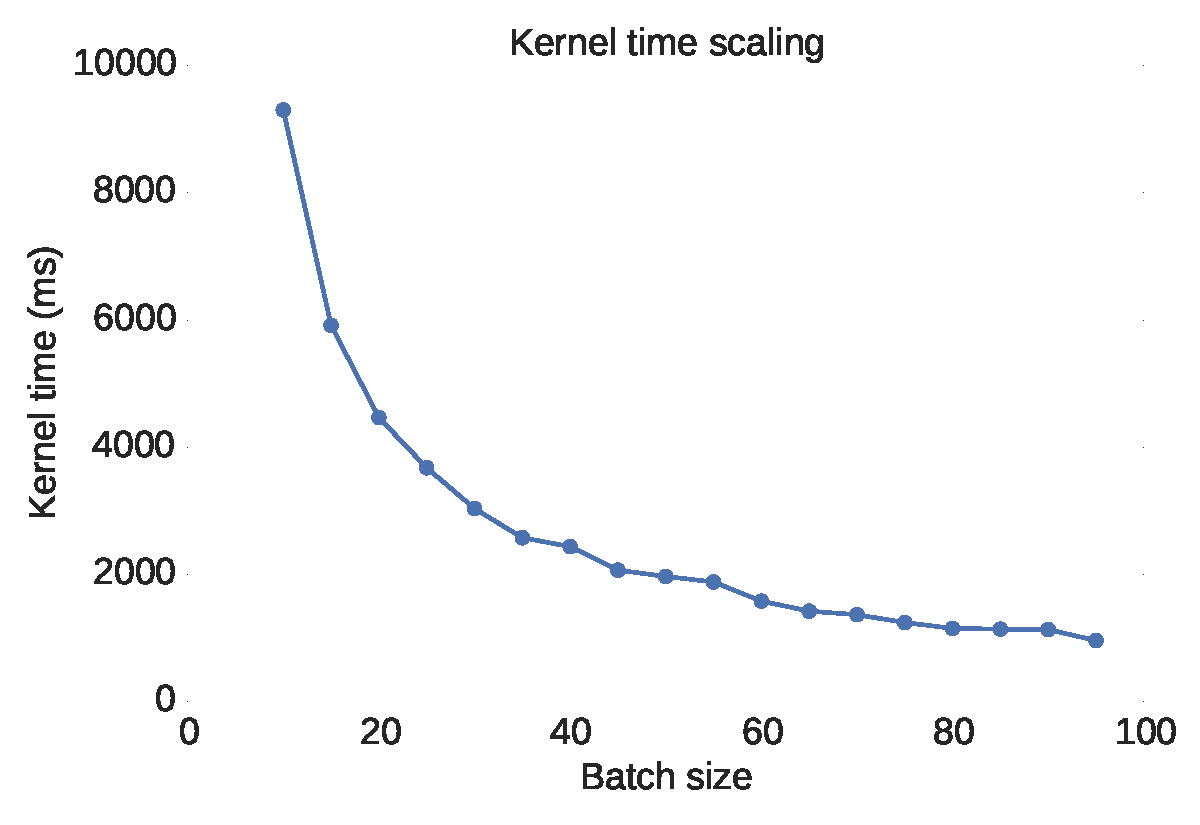
\includegraphics[width=\linewidth]{kernel_time_batch_scaling.pdf}
  \caption{Kernel time as a function of batch size. Here the we used $1000$ samples ($N_s=1000) $ with $3$ features ($N_f=3$). The learning rate $\alpha=0.01$ was set to ensure the convergence of the of all the runs, the data show here is for $1000$ iterations.}
  \label{fig:test_batch_size_kernel}
\endminipage
\hfill
\minipage{0.49\textwidth}
  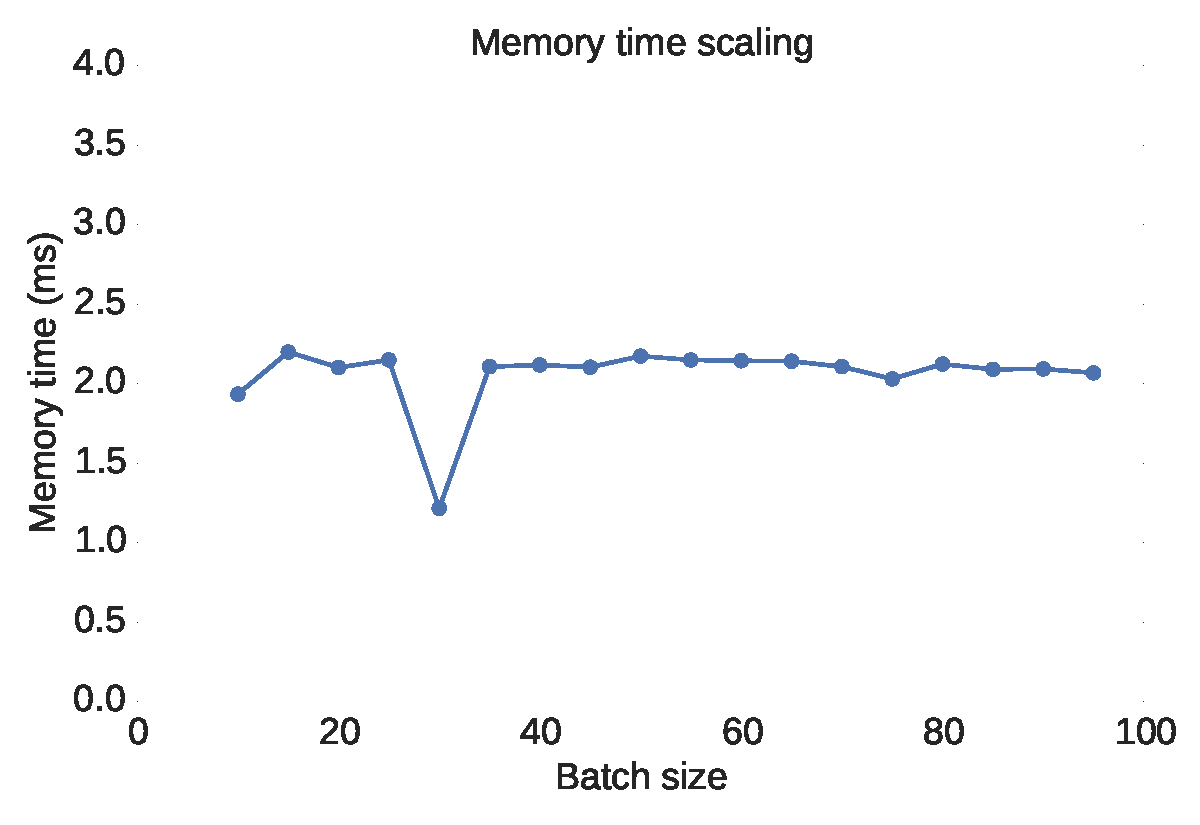
\includegraphics[width=\linewidth]{memory_time_batch_scaling.pdf}
  \caption{Kernel time as a function of batch size. Here the we used $1000$ samples ($N_s=1000) $ with $3$ features ($N_f=3$). The learning rate $\alpha=0.01$ was set to ensure the convergence of the of all the runs, the data show here is for $1000$ iterations.}
  \label{fig:test_batch_size_memory}
\endminipage
\end{figure}

We analyze the accuracy of the algorithm by looking at its performance in terms
of error on the dataset, and how well it was able to approximate the true weights
of the generating process.
We first calculated the \textbf{sum of squared errors} over all the data points, 
this allowed us to have a measure of how well the algorithm is predicting the data. 
As an alternative view, given that we have access to the underlying model we know the 
ground truth  for the weight, which allows us to calculate the difference between 
the true weights or coefficients that were used to generate the data and the ones that
the model estimates. We call this the \textbf{weight error}. In Figure
\ref{fig:test_batch_size_error} we show how for this particular experiment the
error evolves as a function of the batch size. We note that the variation of the errors
is very small and therefore we can claim that at least the algorithm is showing consistent
results independently of the batch size for this dataset. Going further in Figure 
\ref{fig:test_batch_size_werror} we show that the weights the model is predicting
approximate very well the ground truth which means that at least
for this dataset the algorithm is both consistent and accurate. 

%%%%%%%%%%%%%%%%%%%%%%%%%%%
% Errors for batch size 
%%%%%%%%%%%%%%%%%%%%%%%%%%%
\begin{figure}[H]
\minipage{0.49\textwidth}
	\centering
  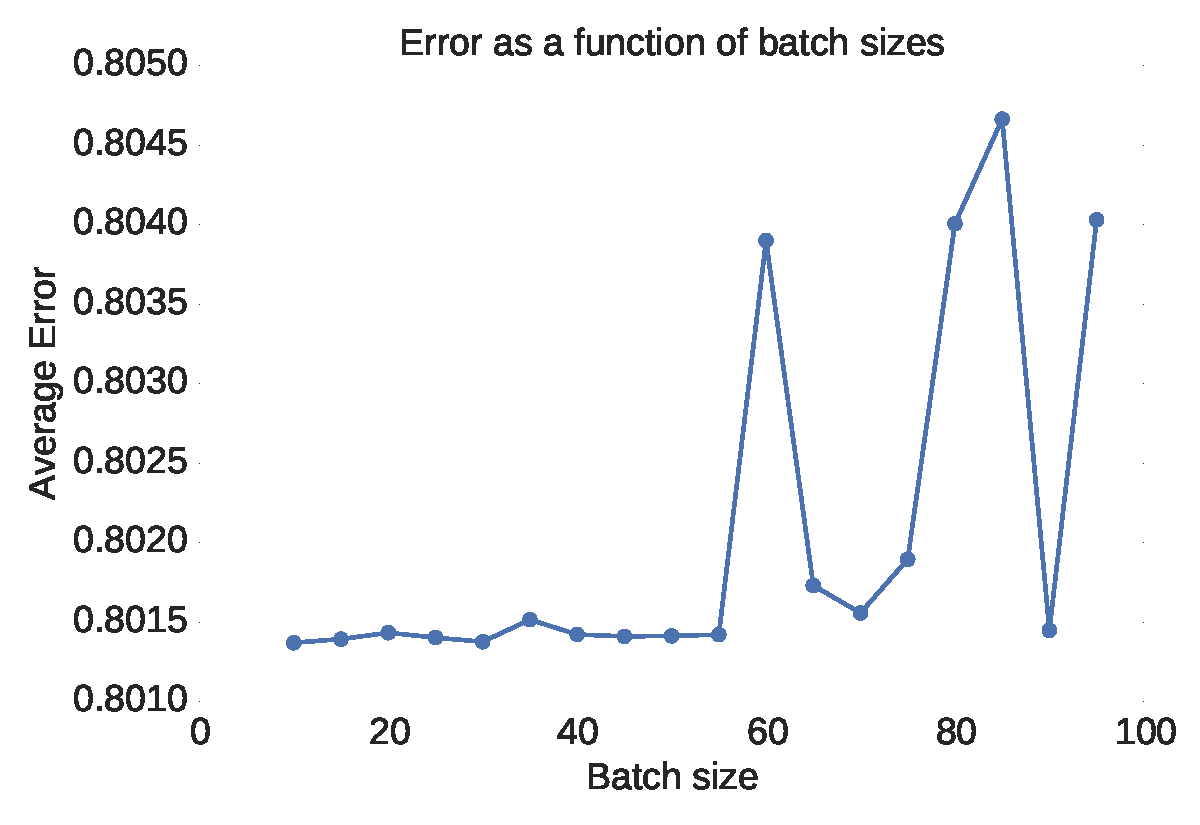
\includegraphics[width=\linewidth]{errors_batch_scaling.pdf}
  \caption{Average error as a function of the batch size. Here the we used $1000$ samples ($N_s=1000$) with $3$ features ($N_f=3$). The learning rate $\alpha=0.01$ was set to ensure the convergence of the of all the runs, the data show here is for $1000$ iterations}
  \label{fig:test_batch_size_error}
\endminipage
\hfill
\minipage{0.49\textwidth}
  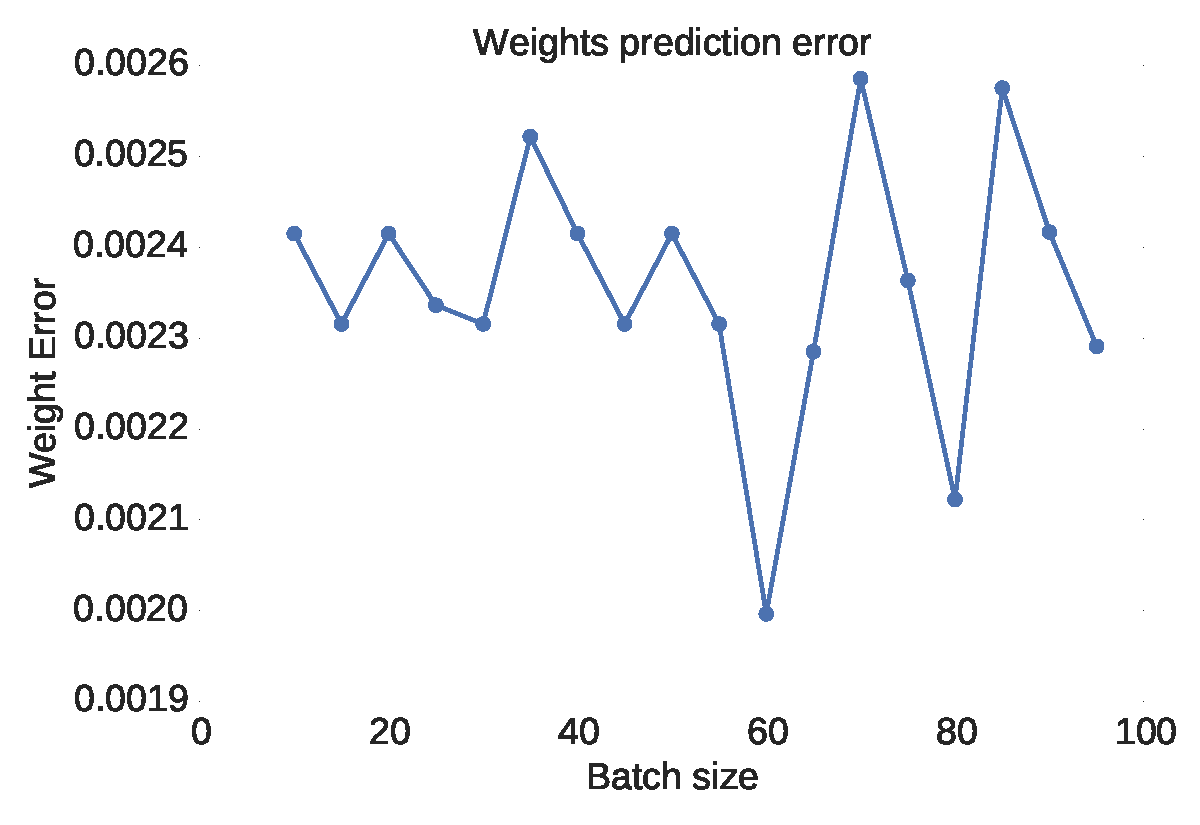
\includegraphics[width=\linewidth]{weights_errors_batch_scaling.pdf}
  \caption{Weight errors as a function of batch size. Here the we used $1000$ samples ($N_s=1000) $ with $3$ features ($N_f=3$). The learning rate $\alpha=0.01$ was set to ensure the convergence of the of all the runs, the data show here is for $1000$ iterations}
  \label{fig:test_batch_size_werror}
\endminipage
\end{figure}

We also tested how the algorithm behaves when we increase the number of
training samples ($N_s$). In Figure \ref{fig:batch_size_scaling_kernel} we show 
how the kernel time scales for different values of $N_s$. 
We can observe that the there is an increase in the kernel time with the 
number of samples as expected, but that the overall scaling behavior is the same. 
The batchsize-bound parallelism is evident here as well, as we observe that the increases in kernel 
time for different number of samples are more pronounced for small batch sizes. 

We illustrate memory time behavior in Figure \ref{fig:batch_size_scaling_memory}. Again, 
we note that there is no variation in the time that it takes to load and transfer the 
data at this scale, as shown previously. However there as we could expect 
there is an effect on it as we increase the quantity of data to load. 

%%%%%%%%%%%%%%%%%%%%%%%%%%%
% Number of samples scaling for batch size
%%%%%%%%%%%%%%%%%%%%%%%%%%%


\begin{figure}[H]
\minipage{0.49\textwidth}
	\centering
  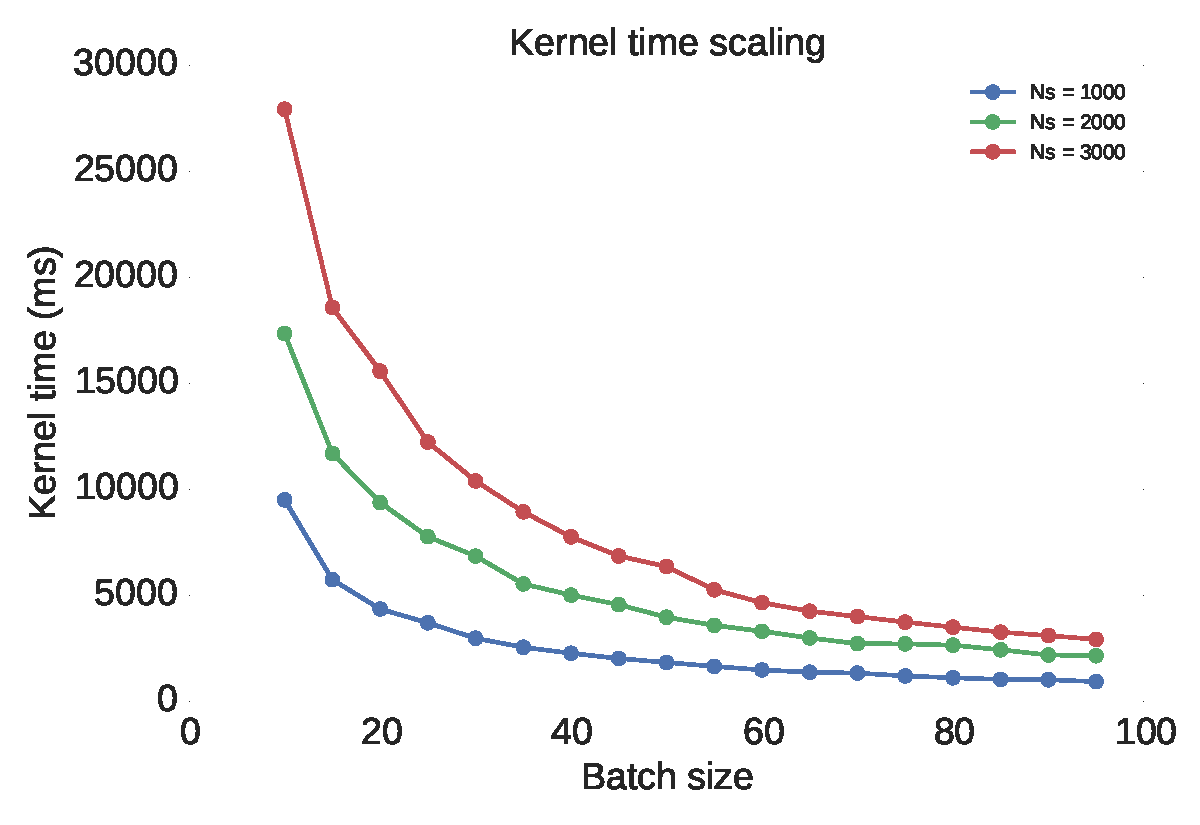
\includegraphics[width=\linewidth]{batch_size_scaling_kernel.pdf}
  \caption{Kernel time as a function of batch size for different sample sizes. Here we used sample sizes ($N_s$) of $1000$, $2000$ and $3000$. Furthermore we used $3$ features ($N_f=3$). The learning rate $\alpha=0.01$ was set to ensure the convergence of the of all the runs, the data show here is for $1000$ iterations.}
  \label{fig:batch_size_scaling_kernel}
\endminipage
\hfill
\minipage{0.49\textwidth}
  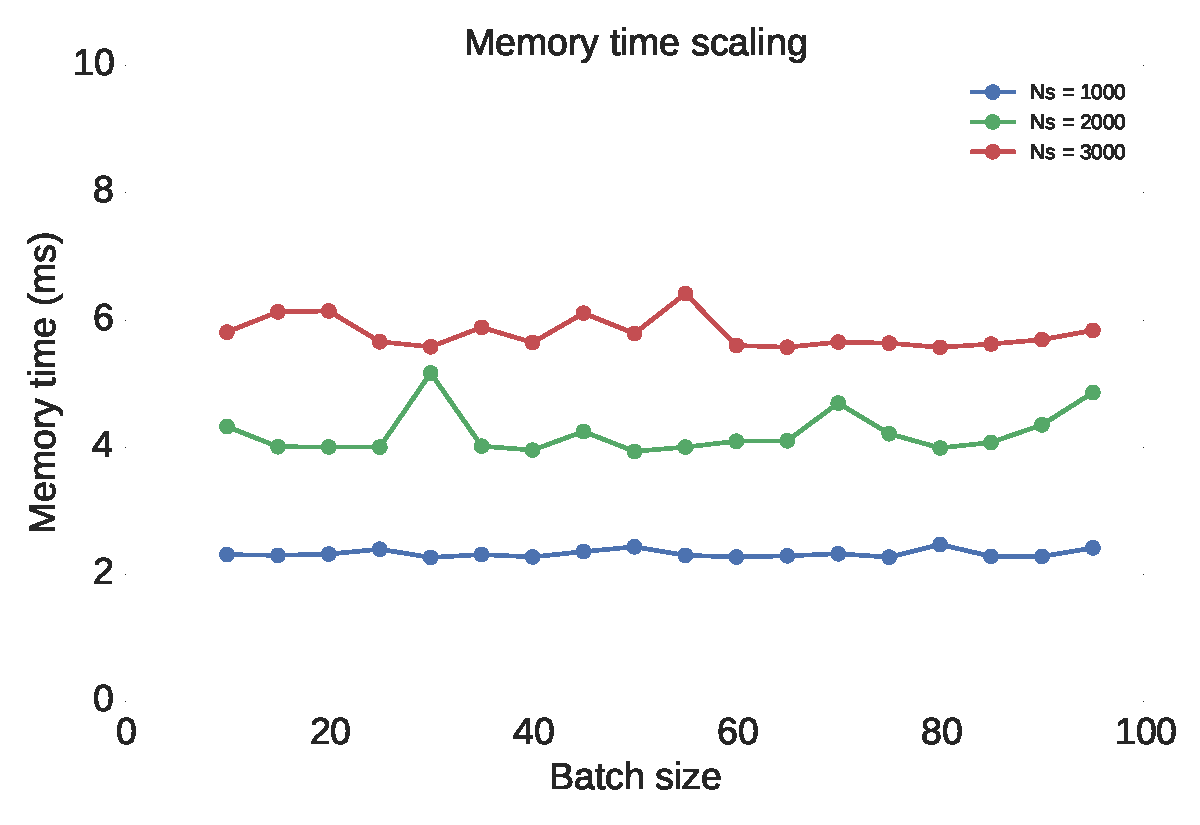
\includegraphics[width=\linewidth]{batch_size_scaling_memory.pdf}
  \caption{Kernel time as a function of batch size for different sample sizes. Here we used sample sizes ($N_s$) of $1000$, $2000$ and $3000$. Furthermore we used $3$ features ($N_f=3$). The learning rate $\alpha=0.01$ was set to ensure the convergence of the of all the runs, the data show here is for $1000$ iterations.}
  \label{fig:batch_size_scaling_memory}
\endminipage
\end{figure}

\subsection{Number of Samples}

In order to test how exactly our algorithm scales with the number of samples 
of the data set ($N_s$) we calculated the kernel time for different subsets 
size of a particular data set. As described in the experiments sections we did
this in order to make the comparison that would change less context. The results
of this are illustrated in figure \ref{fig:n_samples_kernel} where we can appreciate
a linear increase with the sample size. We repeated the process for 
the memory time and we illustrate the results of this experiments 
in figure \ref{fig:n_samples_memory}. In it we can appreciate 
the more chaotic but still linear increase of the memory time as function of the sample size. 

%%%%%%%%%%%%%%%%%%%%%%%%%%%
% Number of samples scaling 
%%%%%%%%%%%%%%%%%%%%%%%%%%%
\begin{figure}[H]
\minipage{0.49\textwidth}
	\centering
  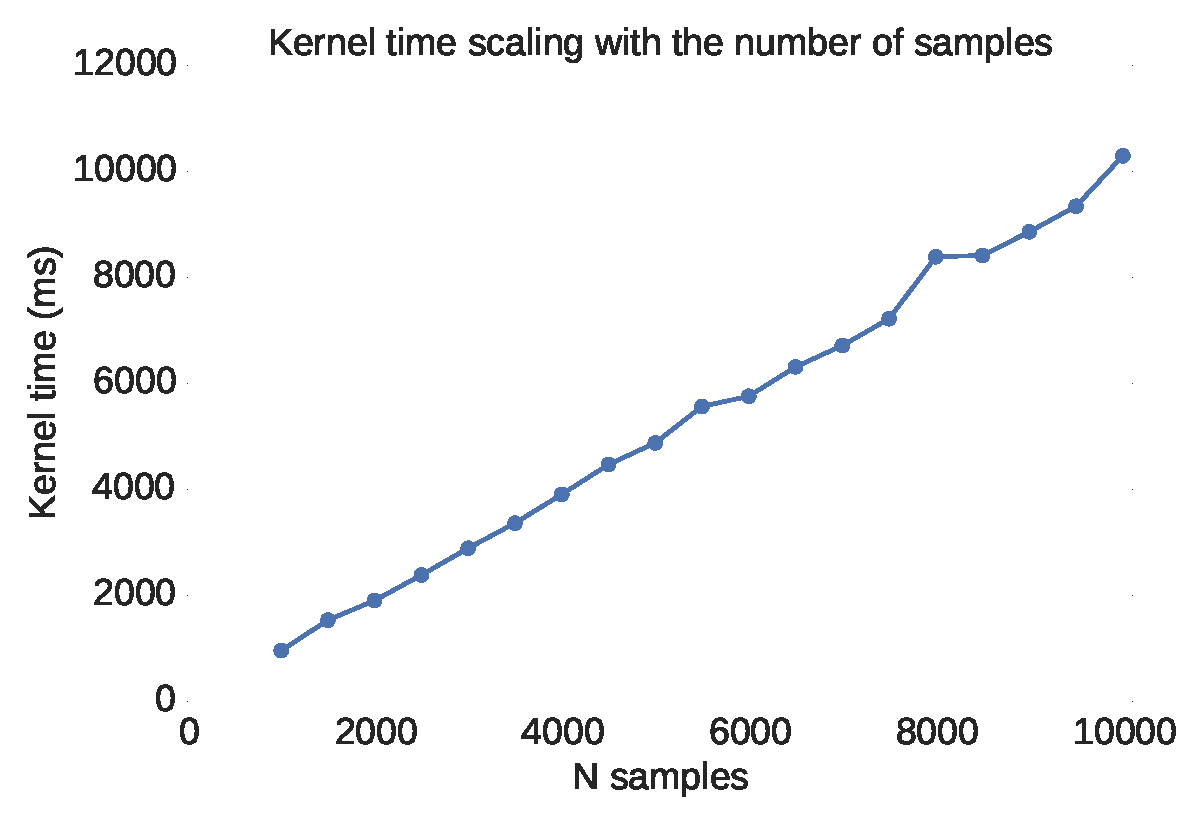
\includegraphics[width=\linewidth]{kernel_time_n_samples.pdf}
  \caption{Kernel time as a function of $N_s$. Here we used a batch size of $100$ Furthermore we used $3$ features ($N_f=3$). The learning rate $\alpha=0.01$ was set to ensure the convergence of the of all the runs, the data show here is for $1000$ iterations.}
  \label{fig:n_samples_kernel}
\endminipage
\hfill
\minipage{0.49\textwidth}
  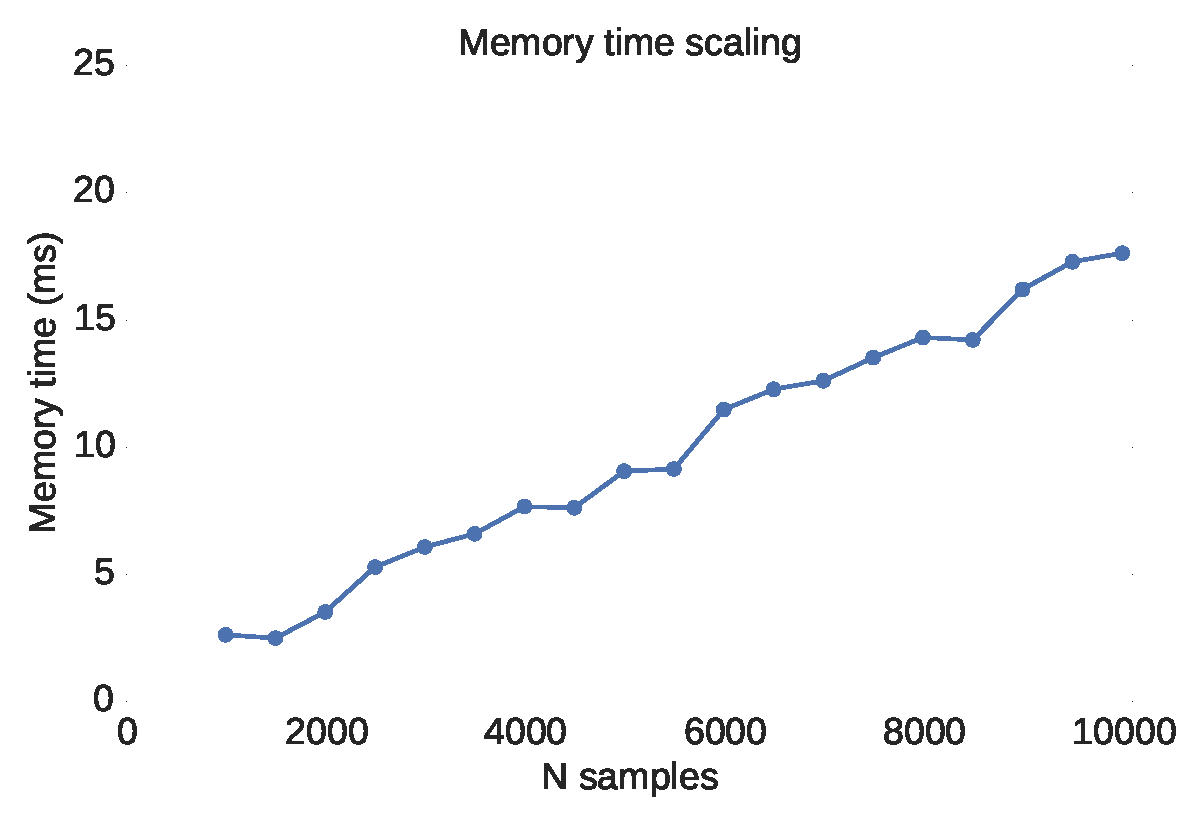
\includegraphics[width=\linewidth]{memory_time_n_samples.pdf}
  \caption{Memory time as a function of $N_s$. Here we used a batch size of $100$ Furthermore we used $3$ features ($N_f=3$). The learning rate $\alpha=0.01$ was set to ensure the convergence of the of all the runs, the data show here is for $1000$ iterations.}
  \label{fig:n_samples_memory}
\endminipage
\end{figure}

In order to do the same sanity check that we did for the batch size scaling we show here how the sum of the squared errors and the weight error changed as a function of the sample size. We present those in figure \ref{fig:n_samples_error} and figure \ref{fig:n_samples_weights_error}. We see a small increase in the errors because the sum is not averaged so every time we add a term we contribute a little bit to this factor, even if the overall magnitude is still small. The weights errors on the other hand are surprisingly consistent which reflect the fact the algorithm converges quite certainly for this particular data set.   

%%%%%%%%%%%%%%%%%%%%%%%%%%%
% Number of samples errors
%%%%%%%%%%%%%%%%%%%%%%%%%%%
\begin{figure}[H]
\minipage{0.49\textwidth}
	\centering
  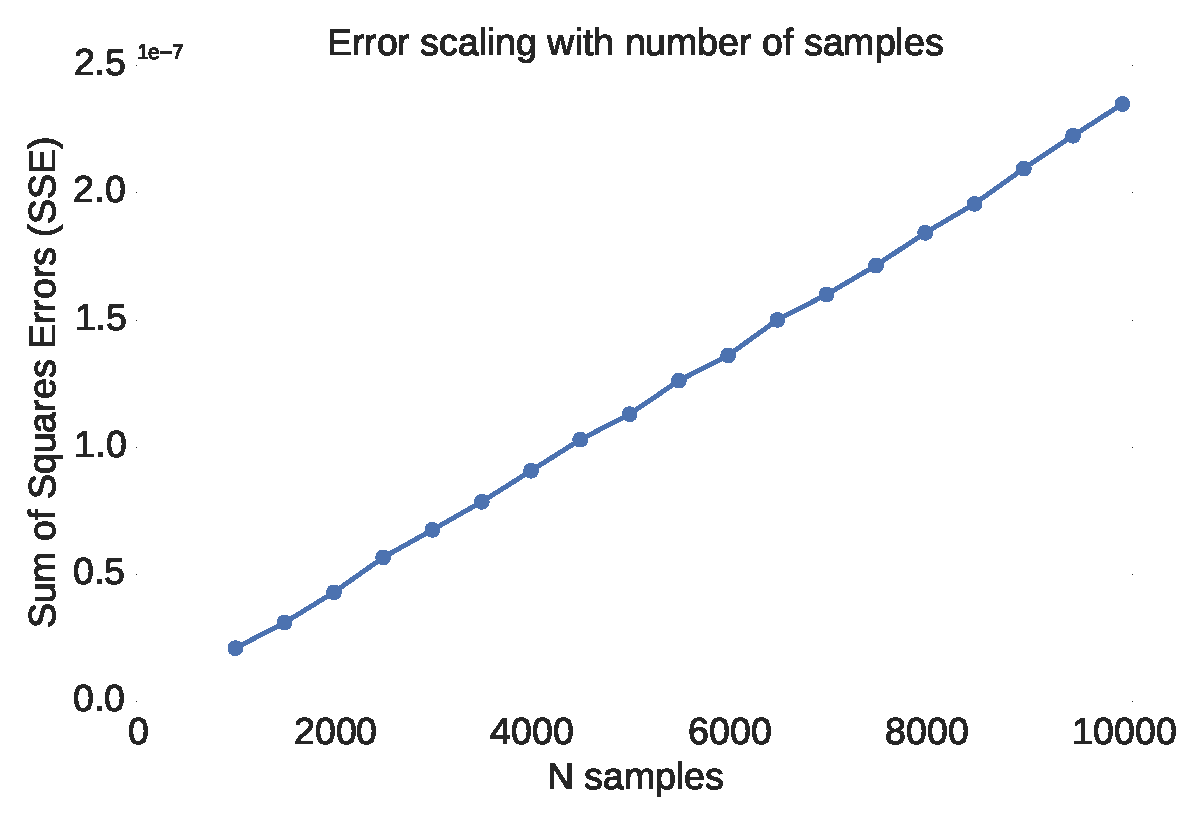
\includegraphics[width=\linewidth]{errors_n_samples.pdf}
  \caption{Kernel time as a function of $N_s$. Here we used a batch size of $100$ Furthermore we used $3$ features ($N_f=3$). The learning rate $\alpha=0.01$ was set to ensure the convergence of the of all the runs, the data show here is for $1000$ iterations.}
  \label{fig:n_samples_error}
\endminipage
\hfill
\minipage{0.49\textwidth}
  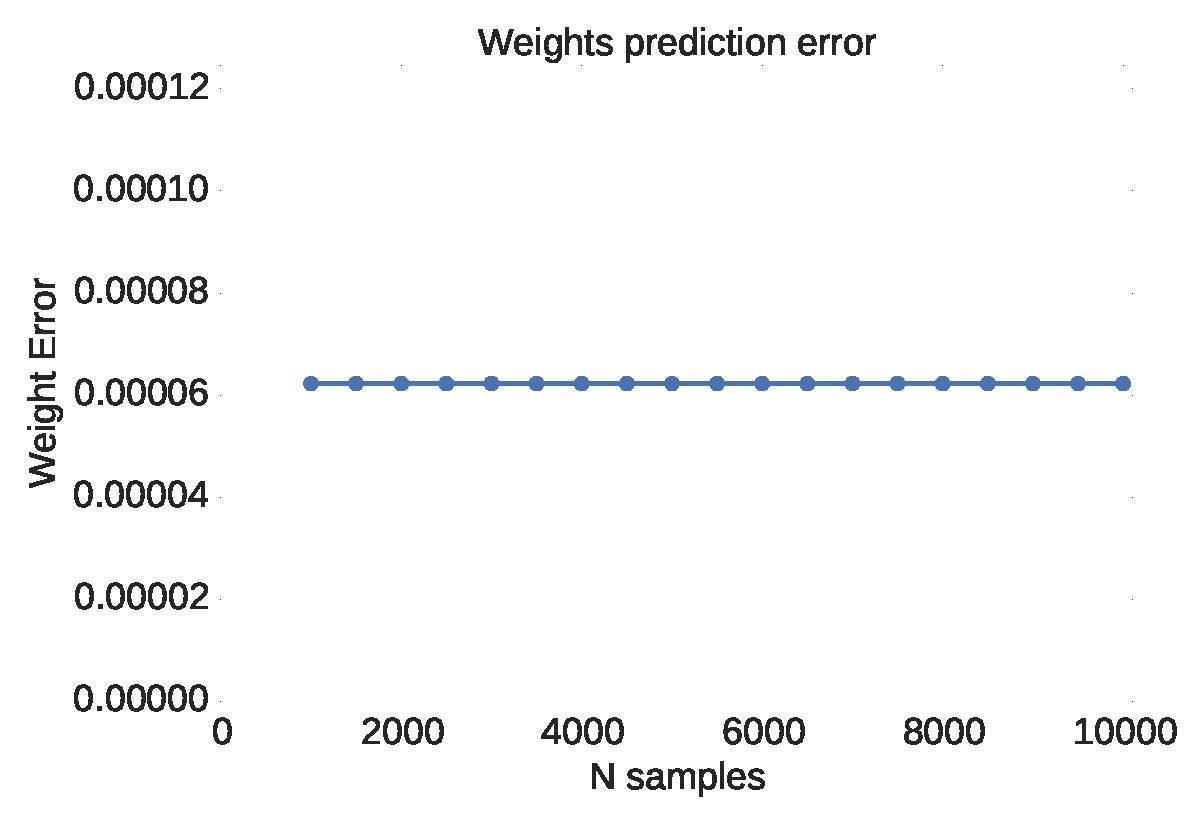
\includegraphics[width=\linewidth]{weights_errors_n_samples.pdf}
  \caption{Memory time as a function of $N_s$. Here we used a batch size of $100$ Furthermore we used $3$ features ($N_f=3$). The learning rate $\alpha=0.01$ was set to ensure the convergence of the of all the runs, the data show here is for $1000$ iterations.}
  \label{fig:n_samples_weights_error}
\endminipage
\end{figure}

\subsection{Number of Features}


\section{Discussion}

The runtime and scaling characteristics that we observed in our experiments are
consistent with our expectations, given the unit of parallelism being tied to the
batch. While parallelization in the order of tens to hundreds of threads, which
is what this unit of parallelism can give us, is acceptable for CPU parallel
programming, the same is not true for GPUs.

In our initial testing we implemented batch (not mini-batch) gradient descent
on the GPU, where we loaded all the data points in the dataset at once, leading
to potentially better parallelism. However since this approach is highly limited
by the amount of memory on the GPU we chose to use mini-batches instead.

The choice of using the batch size as the unit of parallelism was made mostly due to
time constraints, we realize that it is suboptimal and we have the following suggestions
on how to improve the current implementation:

\begin{enumerate}
	\item \textbf{Dynamic Parallelism - cuBLAS for vector operations}
	
	SGD involves a number of vector operations, mostly dot products.
	In the current implementation these are done sequentially through \texttt{for} loops within kernels.
	By using dynamic parallelism and specifically cuBLAS operations
	we can significantly speed up these computations.
	
	
	\item \textbf{Sequential memory access}
	
	In SGD one commonly shuffles the dataset in memory before each iteration, as it has been shown to improve
	convergence performance. In the current implementation we emulate this shuffling by randomizing the
	order in which we access elements of the dataset, leading to non-sequential memory 
	accesses. What we could do instead is to shuffle the data on the GPU memory and perform 
	sequential memory accesses.
	
	\item \textbf{Change parallelism unit}
	
	Perhaps most importantly, in the current implementation our unit of parallelization is the size of the batch; we run one batch 
	at a time and parallelize
	the computations in terms of the data points within the batch. Common batch sizes range from 10 - 1000
	making this way to parallelize highly inefficient on the GPU, even if dynamic parallelism is employed.
	We could change the parallelism scheme of the algorithm so we can run multiple
	batches in parallel, thereby greatly increasing the parallelism and achieving much 
	higher occupancy on the GPU.
\end{enumerate}

During the course of this project we learned a lot about using CUDA and Thrust, and had
to deal with a number of development issues that are common in non-managed memory 
languages like C and C++, a hurdle that was amplified by the need to perform remote
debugging. Despite the cost of development ease however, we also realized the tremendous potential of GPUs for speeding up scientific computations, and will definitely be
using the knowledge we gained by the summer school and this project in our own research.

\bibliographystyle{plainnat}
\bibliography{references}
\end{document}